\documentclass{beamer}
\usepackage{beamerthemesplit}
\usetheme{SPbGU}
%{CambridgeUS}
% Выпишем часть возможных стилей, некоторые из них могут содержать
% дополнительные опции
% Darmstadt, Ilmenau, CambridgeUS, default, Bergen, Madrid, AnnArbor,Pittsburg, Rochester,
% Antiles, Montpellier, Berkley, Berlin
\usepackage{pdfpages}
\usepackage{amsmath}
\usepackage{cmap} % for serchable pdf's
\usepackage[T2A]{fontenc} 
\usepackage[utf8]{inputenc}
\usepackage[english,russian]{babel}
\usepackage{indentfirst}
\usepackage{amsmath}
\usepackage{dot2texi}
\usepackage{tikz}
\usepackage{fancyvrb}
\usepackage{graphicx}
\usepackage{array}
%\usepackage{animate}
\usepackage{multimedia}

%\usepackage[usenames,dvipsnames]{color}
\usetikzlibrary{shapes,arrows}
% Если у вас есть логотип вашей кафедры, факультета или университета, то
% его можно включить в презентацию.

%\usefoottemplate{\vbox{}}%  \tinycolouredline{structure!25}% {\color{white}\textbf{\insertshortauthor\hfill% \insertshortinstitute}}% \tinycolouredline{structure}% {\color{white}\textbf{\insertshorttitle}\hfill}% }}

%\logo{
\includegraphics[width=1cm]{SPbGU_Logo.png}}

\title[]{Лексический анализ динамически формируемых строковых выражений}
\institute[СПбГУ]{
Санкт-Петербургский государственный университет}

\author[Полубелова Марина]{Полубелова Марина}

\date{12 ноября 2015г.}

\begin{document}

\begin{frame}
    \begin{tabular}[c c c]{m{2cm} m{5.5cm} m{3cm}}
        \begin{center}
        
\includegraphics[width=1.3cm]{SPbGU_Logo.png}
    \end{center}
    &
    Третья международная научно-практическая конференция: \newline Инструменты и методы анализа программ, ТМPА-2015
    \newline
    12--14 ноября, Санкт-Петербург
    &
    \begin{center}
        
\includegraphics[width=3cm]{tmpa2015_logo.png}
    \end{center}
    \\
    &&
    \end{tabular}
    \titlepage
\end{frame}


\definecolor{green}{RGB}{0, 100, 0}
\definecolor{orange}{RGB}{255,110,0}
\definecolor{gray}{RGB}{105,105,105}
\begin{frame}[fragile]
\transwipe[direction=90]
\frametitle{Примеры}
\begin{itemize}

\item Встроенный SQL в С\#
\begin{Verbatim}[commandchars=\\\{\}]
\textcolor{green}{private void} \textcolor{blue}{Go} (\textcolor{blue}{int} cond)\{
	\textcolor{blue}{string} columnName = cond > \textcolor{gray}{3} ? \textcolor{red}{"X"}:(cond < \textcolor{gray}{0} ? \textcolor{red}{"Y"}:\textcolor{red}{"Z"});
	\textcolor{blue}{string} queryString = 
	             \textcolor{red}{"SELECT name"} + columnName + \textcolor{red}{" FROM table"};
	Program.ExecuteImmediate(queryString);
\}
\end{Verbatim}
		
\item Динамически генерируемый HTML в PHP-программах
\begin{Verbatim}[commandchars=\\\{\}]	
<?php 
    \$name = \textcolor{red}{'your name'};
    echo \textcolor{red}{'<table>} 
         \textcolor{red}{<tr><th>Name</th></tr>}  
         \textcolor{red}{<tr><td>'}.\$name.\textcolor{red}{'</td></tr>} 
         \textcolor{red}{</table>'};
?>
\end{Verbatim}
\end{itemize}
\end{frame}


\begin{frame}
\transwipe[direction=90]
\frametitle{Мотивация}
Использование динамически формируемых строковых выражений:
\begin{itemize}
\item уменьшает надежность
\begin{itemize}
\item нет статического поиска ошибок
\end{itemize}
\item увеличивает уязвимость
\begin{itemize}
\item SQL инъекции
\item межсайтовый скриптинг
\end{itemize}
\end{itemize}
\end{frame}


\begin{frame}
\transwipe[direction=90]
\frametitle{Статический анализ программ}
%Классический подход:
\begin{itemize}
\item Лексический анализ
\item Синтаксический анализ 
\item Семантический анализ
\end{itemize}

%\textbf{Автоматизированный} способ создания лексических и синтаксических анализаторов:
%\begin{itemize}
%\item Lex
%\item Yacc и др.
%\end{itemize}
\end{frame}


\begin{frame}
\transwipe[direction=90]
\frametitle{Обзор существующих инструментов}
\begin{itemize}
\item Проверка выражения на соответствие описанию некоторой эталонной грамматики
\begin{itemize}
\item Java String Analyzer
\item PHP String Analyzer
\item Alvor
\end{itemize}

\item Статический анализ программы на уязвимость
\begin{itemize}
\item Pixy
\item Stranger
\item SAFELI
\end{itemize}
\end{itemize}
\end{frame}

\begin{frame}
\transwipe[direction=90]
\frametitle{Генераторы лексических анализаторов}

\textbf{Автоматизированный} способ создания лексических и синтаксических анализаторов:
\begin{itemize}
\item Lex
\item Yacc и др.
\end{itemize}
\end{frame}

\begin{frame}
\transwipe[direction=90]
\frametitle{Проект YaccConstructor}
\begin{itemize}
\item YaccConstructor --- модульный инструмент, предназначенный для проведения лексического анализа и синтаксического разбора
\item YaccConstructor --- платформа для поддержки встроенных языков
\newline
\item Не поддерживаются циклы и строковые операции
\end{itemize}
\end{frame}


\begin{frame}
\transwipe[direction=90]
\frametitle{Постановка задачи}
\textbf{Цель}: разработать автоматизированный подход создания лексического анализатора для динамически формируемого кода

\begin{itemize}
\item разработать алгоритм лексического анализа выражений, формируемых с помощью строковых операций и циклов
\item реализовать генератор лексических анализаторов
\item сохранить привязку лексических единиц к исходному коду
\end{itemize}
\end{frame}

\begin{frame}[fragile]
\transwipe[direction=90]
\frametitle{Аппроксимация}
\begin{itemize}
\item 
\begin{Verbatim}[commandchars=\\\{\}]
\textcolor{green}{private void} \textcolor{blue}{Go} (\textcolor{blue}{int} cond)\{
	\textcolor{blue}{string} columnName = cond > \textcolor{gray}{3} ? \textcolor{red}{"X"}:(cond < \textcolor{gray}{0} ? \textcolor{red}{"Y"}:\textcolor{red}{"Z"});
	\textcolor{blue}{string} queryString = 
	             \textcolor{red}{"SELECT name"} + columnName + \textcolor{red}{" FROM table"};
	Program.ExecuteImmediate(queryString);
\}
\end{Verbatim}

\item Множество значений:\\ 		
\{ "SELECT nameX FROM table"; "SELECT nameY FROM table"; "SELECT nameZ FROM table" \}

		
\item Результат аппроксимации:
\begin{center}
	{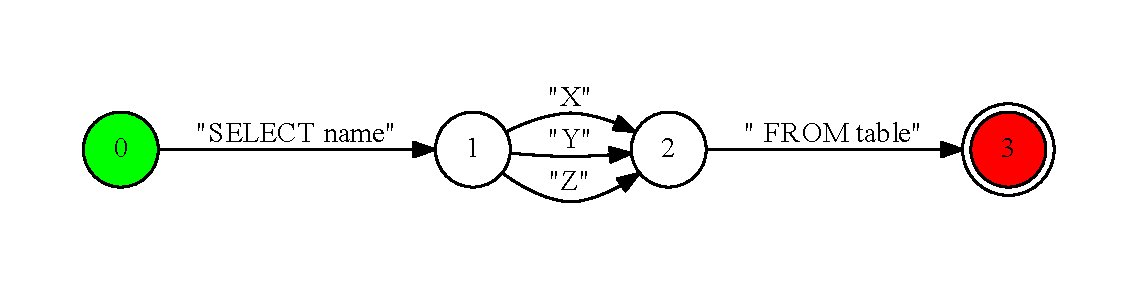
\includegraphics[width=1.0\linewidth]{tsql_test}}
\end{center}

\end{itemize}
\end{frame}


\begin{frame}
\transwipe[direction=90]
\frametitle{Лексический анализ строковых выражений}
\begin{itemize}
\item На вход анализатору подается конечный автомат, полученный в результате аппроксимации множества значений строкового выражения
\item На выходе получаем либо конечный автомат над токенами, либо список лексических ошибок. Токен содержит в себе:
	\begin{itemize}
	\item идентификатор токена
	\item конечный автомат, описывающий все возможные последовательности символов для данного токена
	\end{itemize}
\end{itemize}

\begin{block}{}
\textbf{Задача лексического анализа}: получение конечного автомата над алфавитом токенов эталонной грамматики из конечного автомата над алфавитом символов обрабатываемого языка
\end{block}

\end{frame}

\begin{frame}[fragile]
\transwipe[direction=90]
\frametitle{Пример}
\begin{itemize}
\item 
\begin{Verbatim}[commandchars=\\\{\}]
\textcolor{green}{private void} \textcolor{blue}{Go} (\textcolor{blue}{int} cond)\{
	\textcolor{blue}{string} columnName = cond > \textcolor{gray}{3} ? \textcolor{red}{"X"}:(cond < \textcolor{gray}{0} ? \textcolor{red}{"Y"}:\textcolor{red}{"Z"});
	\textcolor{blue}{string} queryString = 
	             \textcolor{red}{"SELECT name"} + columnName + \textcolor{red}{" FROM table"};
	Program.ExecuteImmediate(queryString);
\}
\end{Verbatim}
		
\item Результат аппроксимации:
\begin{center}
	{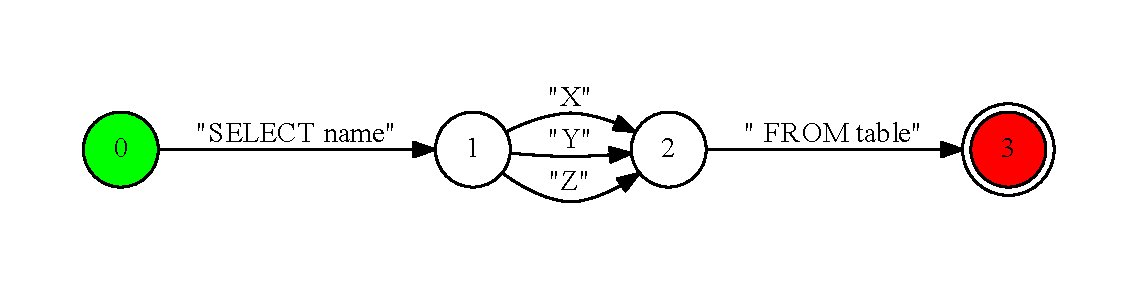
\includegraphics[width=1.0\linewidth]{tsql_test}}
\end{center}

\item Результат лексического анализа:
\begin{center}
    {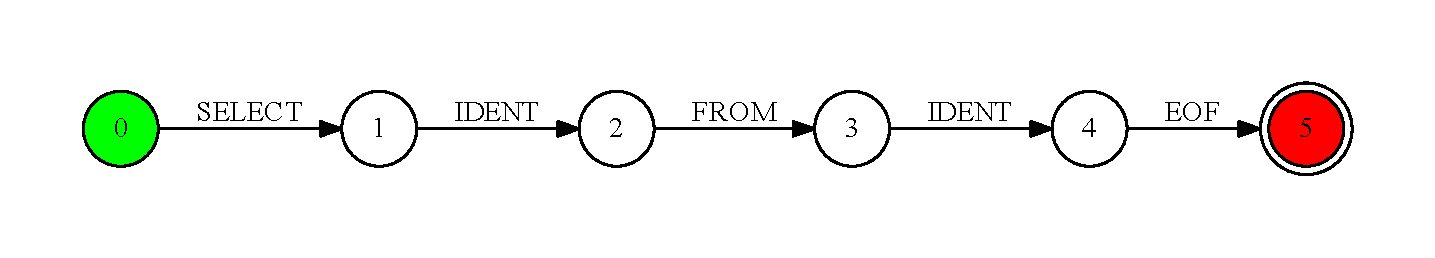
\includegraphics[width=1.0\linewidth]{tsql_test_appr}}
\end{center}
\end{itemize}
\end{frame}


\begin{frame}[fragile]
\transwipe[direction=90]
\frametitle{Пример}
\begin{itemize}
\item Результат лексического анализа:
	\begin{center}
        {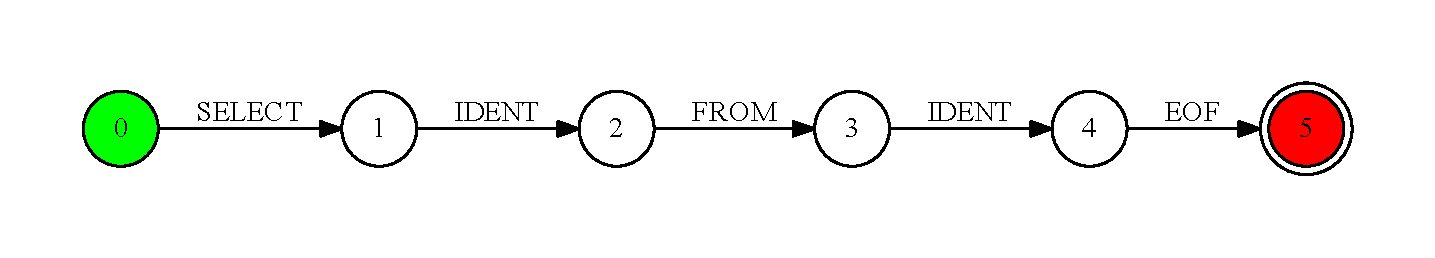
\includegraphics[width=1.0\linewidth]{tsql_test_appr}}
    \end{center}
		
\item Конечный автомат первого токена \verb|IDENT|:
	\begin{center}
        {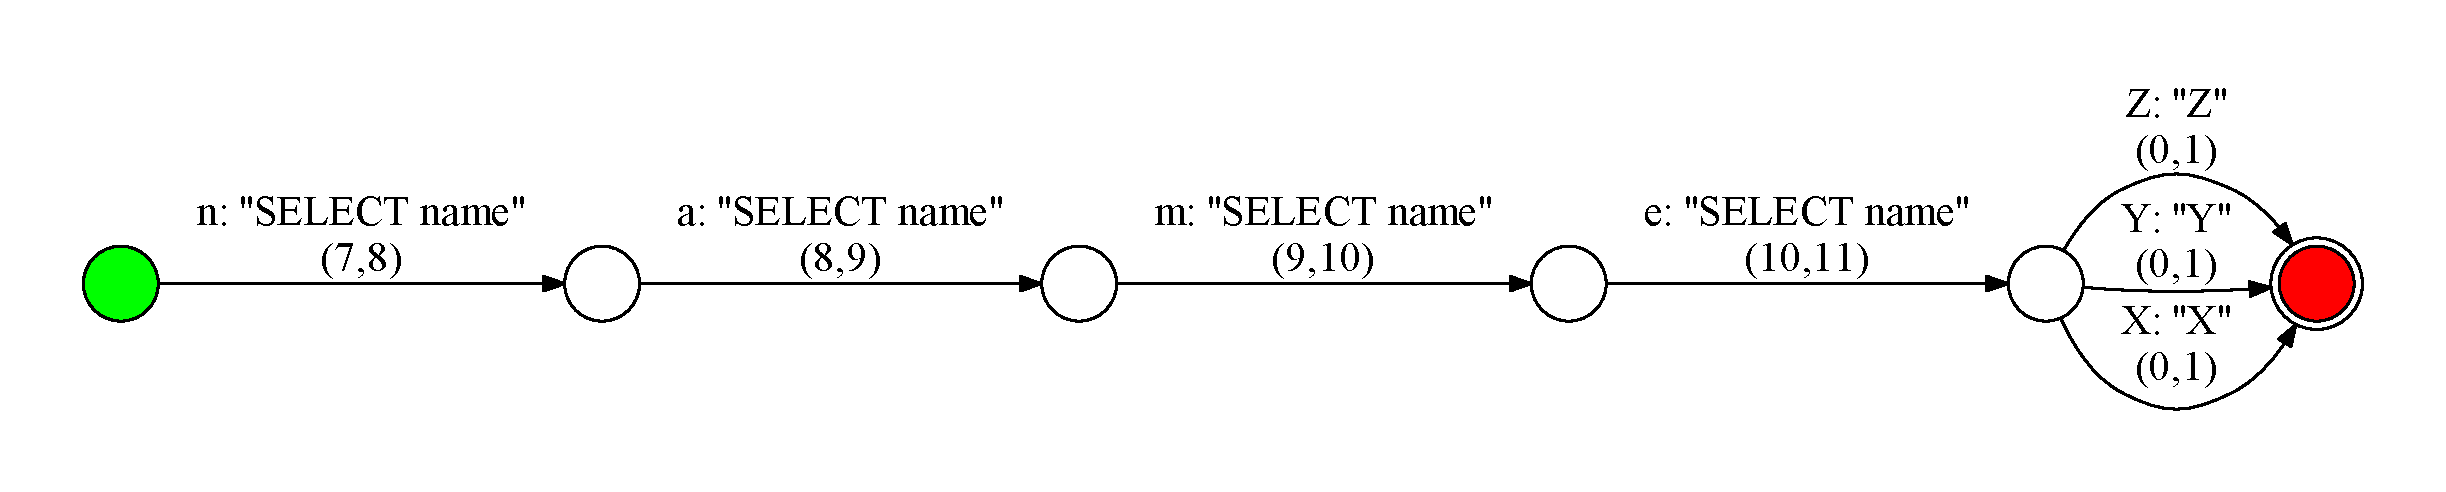
\includegraphics[width=1.0\linewidth]{tsql_ident_1}}
    \end{center}

\item Конечный автомат второго токена \verb|IDENT|:
	\begin{center}
        {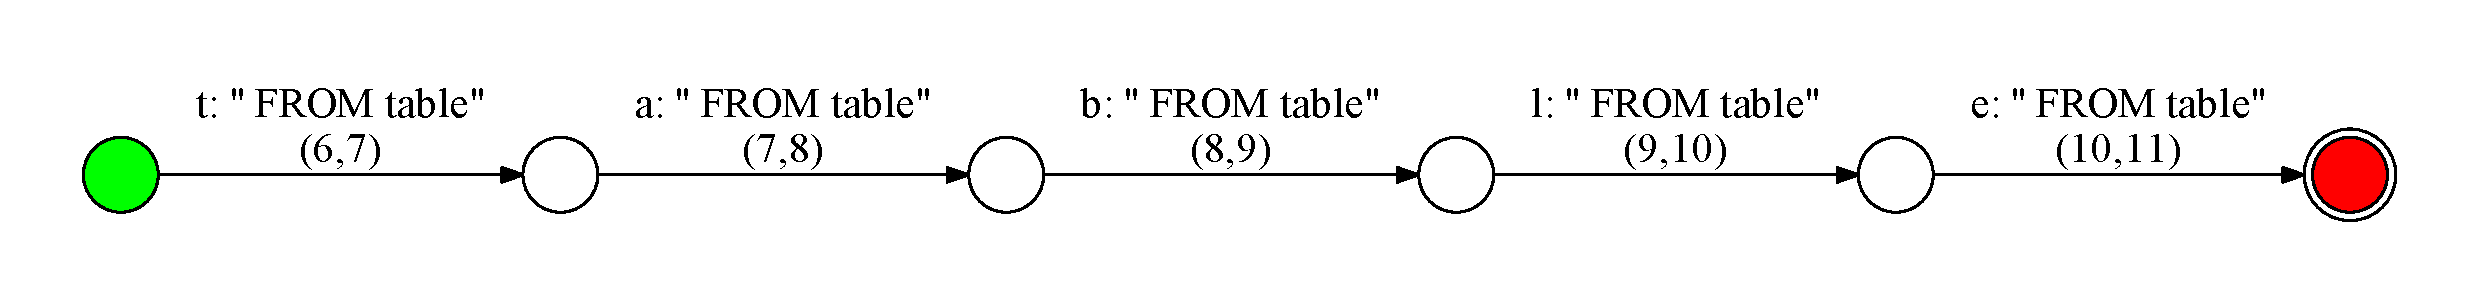
\includegraphics[width=1.0\linewidth]{tsql_ident_2}}
    \end{center}
\end{itemize}
\end{frame}


\begin{frame}[fragile]
\transwipe[direction=90]
\frametitle{Конечный преобразователь}
\begin{itemize}
\item \textbf{Конечный преобразователь} --- это конечный автомат, который может выводить конечное число символов для каждого входного символа

\item \textbf{Композиция} конечных преобразователей --- это два последовательно взаимодействующих конечных преобразователя: выход первого конечного преобразователя является входом для второго конечного преобразователя
\end{itemize}
\end{frame}


\begin{frame}[fragile]
\transwipe[direction=90]
\frametitle{Генератор лексических анализаторов}
\underline{Вход}: \\ 
\begin{itemize}
\item Лексическая спецификация языка
\begin{verbatim}
let digit = ['0'-'9']
let whitespace = [' ' '\t' '\r' '\n']
let num = ['-']? digit+ ('.'digit+)? (['e' 'E'] digit+)?
\end{verbatim}
\begin{tabular}{l | r}
\begin{minipage}{.4\textwidth} 
\footnotesize 
\begin{Verbatim}[commandchars=\\\{\}]
rule token = parse
| whitespace { token lb }
| num  \{ \textcolor{blue}{NUMBER}(lexeme lb) \}
| \textcolor{red}{'-'}  \{ \textcolor{blue}{MINUS}(lexeme lb) \}
| \textcolor{red}{'/'}  \{ \textcolor{blue}{DIV}(lexeme lb) \}
| \textcolor{red}{'+'}  \{ \textcolor{blue}{PLUS}(lexeme lb) \}
| \textcolor{red}{"**"} \{ \textcolor{blue}{POW}(lexeme lb) \}
| \textcolor{red}{'*'}  \{ \textcolor{blue}{MULT}(lexeme lb) \}
\end{Verbatim}
\normalsize
\end{minipage}
&
\begin{minipage}{.4\textwidth}
 \footnotesize 
\begin{Verbatim}[commandchars=\\\{\}]
rule token = parse
| whitespace \{ \textcolor{green}{None} \}
| num  \{ \textcolor{green}{Some}(\textcolor{blue}{NUMBER}(gr)) \}
| \textcolor{red}{'-'}  \{ \textcolor{green}{Some}(\textcolor{blue}{MINUS}(gr)) \}
| \textcolor{red}{'/'}  \{ \textcolor{green}{Some}(\textcolor{blue}{DIV}(gr)) \}
| \textcolor{red}{'+'}  \{ \textcolor{green}{Some}(\textcolor{blue}{PLUS}(gr)) \}
| \textcolor{red}{"**"} \{ \textcolor{green}{Some}(\textcolor{blue}{POW}(gr)) \}
| \textcolor{red}{'*'}  \{ \textcolor{green}{Some}(\textcolor{blue}{MULT}(gr)) \}
\end{Verbatim} 
\normalsize
\end{minipage} \\
\hline 
%\end{tabular}

%\begin{tabular}{c | c}
\begin{minipage}{.4\textwidth}
\begin{center}
 \footnotesize FsLex 
 \normalsize
 \end{center}
\end{minipage}
&
\begin{minipage}{.4\textwidth}
\begin{center}
 \footnotesize YaccConstructor 
 \normalsize
 \end{center}
\end{minipage}
\end{tabular}

\item Описание токенов
\end{itemize}

\underline{Выход}: Описание конечного преобразователя и вспомогательные функции
\end{frame}

\begin{frame}[fragile]
\transwipe[direction=90]
\frametitle{Алгоритм лексического анализа}
\begin{itemize}
\item \textbf{Этап 0}. \\
\underline{Вход}: конечный автомат, полученный в результате построения аппроксимации \\
\underline{Выход}: конечный преобразователь, построенный из входного конечного автомата
\end{itemize}

\begin{tabular}{l r}
     \begin{minipage}{.35\textwidth} 
     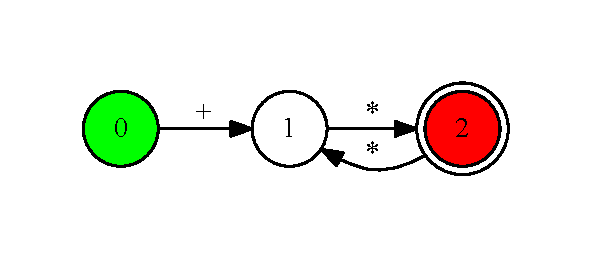
\includegraphics[width=\linewidth]{calc_ex}
     \end{minipage}  
     & 
	\begin{minipage}{.55\textwidth}    
	 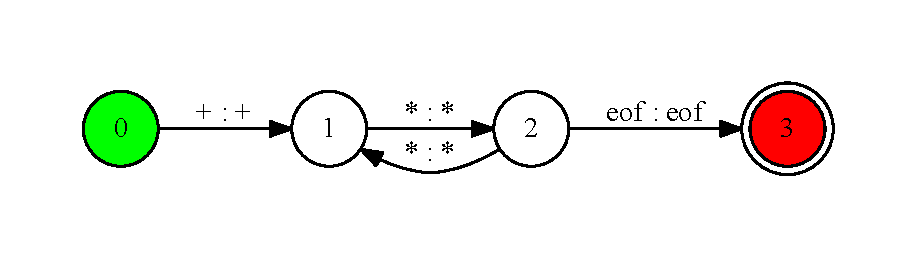
\includegraphics[width=\linewidth]{calc_ex_fst}
	\end{minipage} \\
\end{tabular} 
\end{frame}

\begin{frame}[fragile]
\transwipe[direction=90]
\frametitle{Алгоритм лексического анализа}
\begin{itemize}
\item \textbf{Этап 1}.\\
\underline{Вход}: \\ 
\begin{itemize}
\item конечный преобразователь, полученный на Этапе 0
\item конечный преобразователь, полученный из описания, построенного генератором лексических анализаторов
\end{itemize}
\underline{Выход}: конечный преобразователь над алфавитом токенов и набор лексических ошибок

%\underline{Как}: применение операции композиции над двумя входными конечными преобразователями
\end{itemize}

\begin{center}
 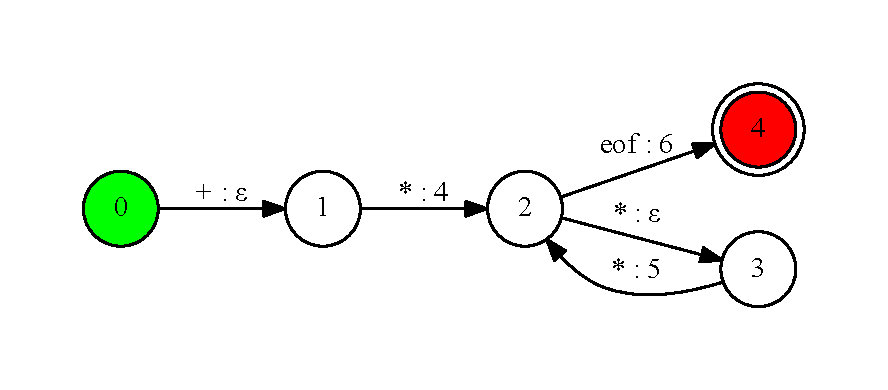
\includegraphics[width=0.6\linewidth]{calc_ex_compose}
\end{center} 

\end{frame}

\begin{frame}[fragile]
\transwipe[direction=90]
\frametitle{Алгоритм лексического анализа}
\begin{itemize}
\item \textbf{Этап 2}. Интерпретация конечного преобразователя \\
\underline{Вход}: конечный преобразователь, полученный на Этапе 1 \\
\underline{Выход}: конечный автомат над алфавитом токенов эталонной грамматики \\
\end{itemize}

\begin{center}	 	
    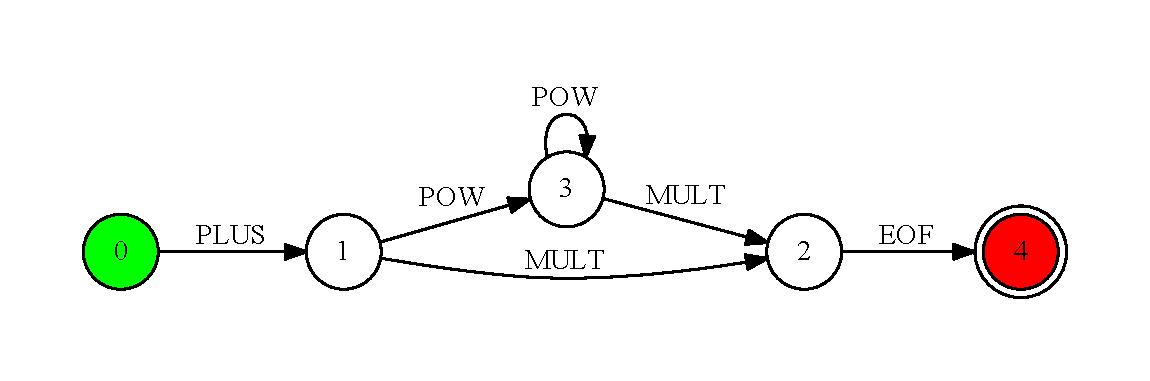
\includegraphics[width=0.8\linewidth]{calc_ex_res}    
\end{center} 
\end{frame}

\begin{frame}
\transwipe[direction=90]
\frametitle{Архитектура инструмента}
\begin{center}
   {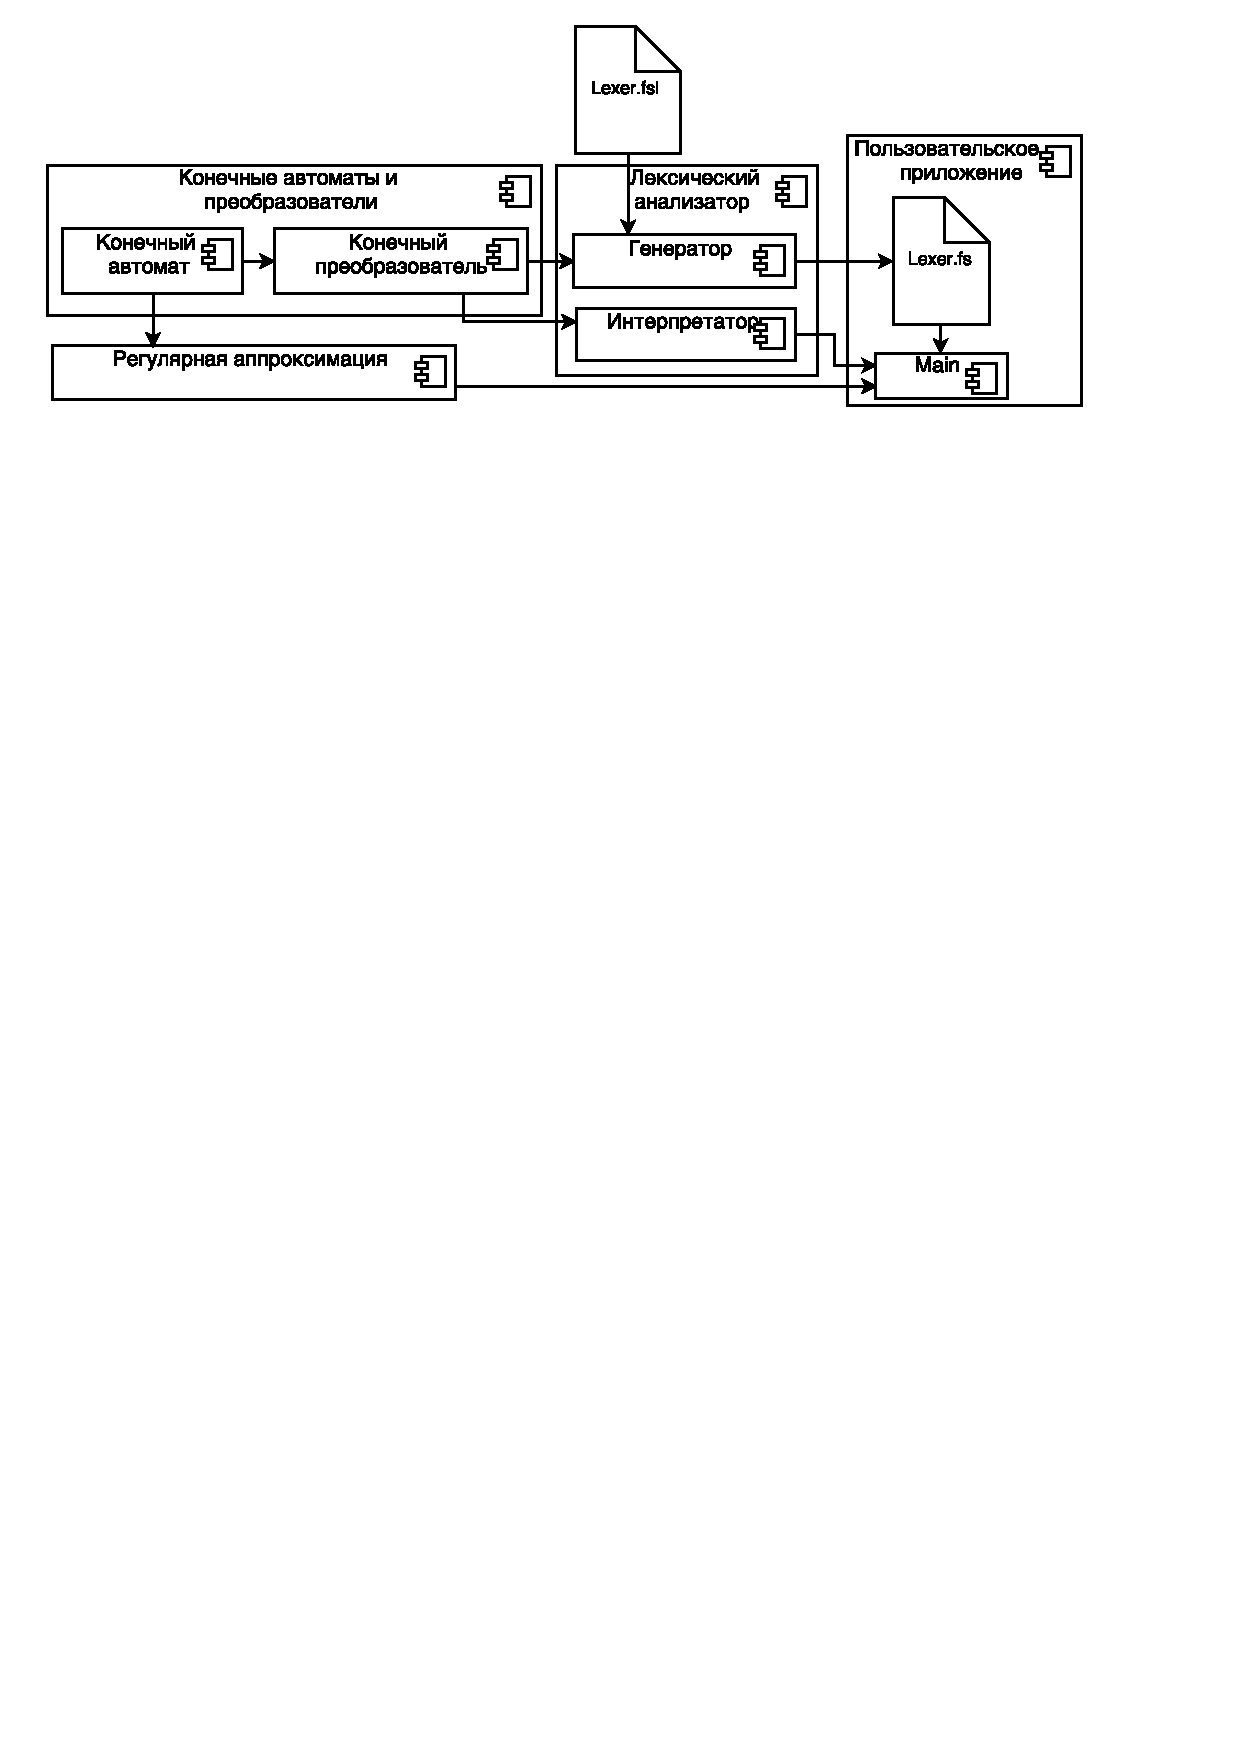
\includegraphics[width=1.0\linewidth]{LexerArch}}
\end{center}
\end{frame}


\begin{frame}[fragile]
\transwipe[direction=90]
\frametitle{Пример 1}
\begin{itemize}
\item \begin{Verbatim}[commandchars=\\\{\}]
\textcolor{green}{private void} \textcolor{blue}{Go} (\textcolor{blue}{int} number)\{
	\textcolor{blue}{string} query =
		         \textcolor{red}{"SELECT nameX FROM tableY WHERE x < "};
	\textcolor{green}{while}(query.Length < number)\{ query += \textcolor{red}{"+ 1 "};\} 
	Program.ExecuteImmediate(query);
\}
\end{Verbatim}

\item Результат аппроксимации: 
\begin{center}
   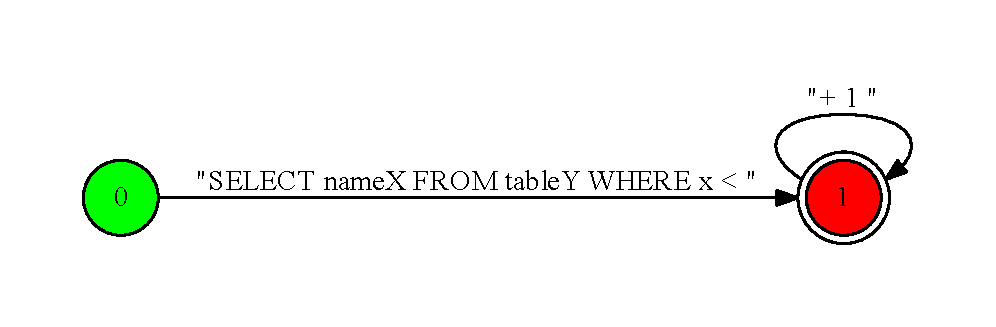
\includegraphics[width=.6\linewidth]{while_appr}
\end{center}
\item Результат лексического анализа: \\
\begin{center}
   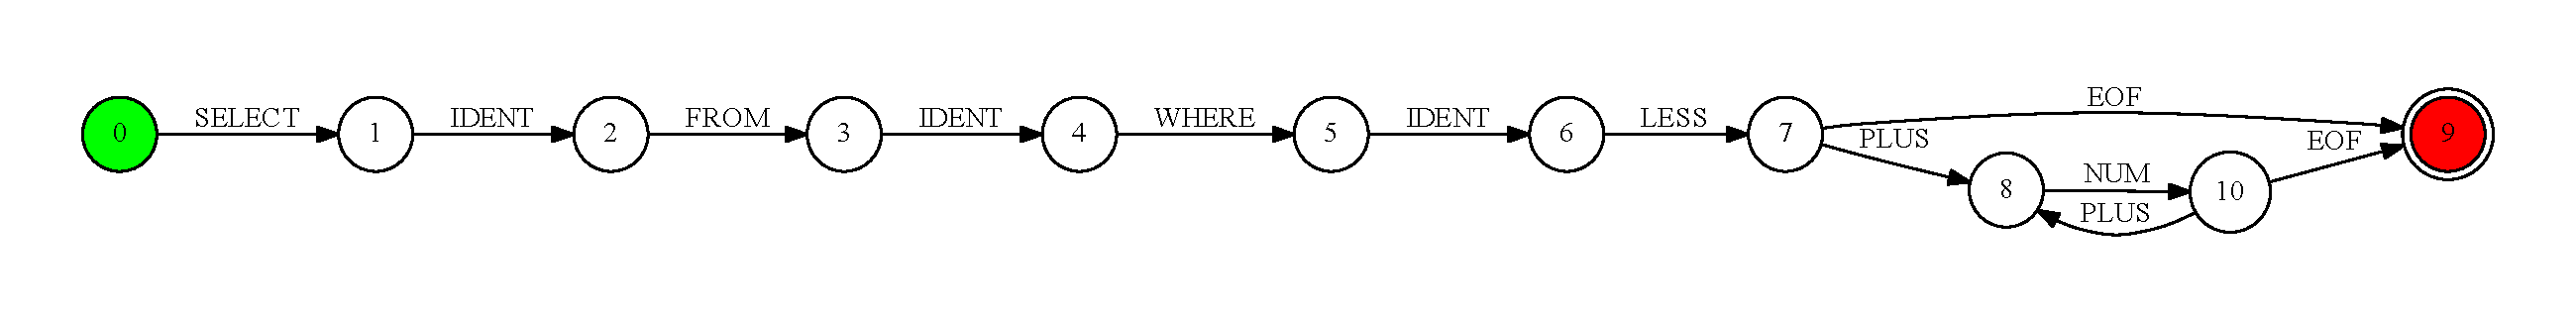
\includegraphics[width=1.0\linewidth]{WhileEx}
\end{center}
\end{itemize}
\end{frame}

\begin{frame}[fragile]
\transwipe[direction=90]
\frametitle{Пример 2}
\begin{itemize}
\item \begin{Verbatim}[commandchars=\\\{\}]
\textcolor{blue}{string} query = \textcolor{red}{"SELECT name"};
\textcolor{green}{for}(int i = 0; i < 10; i++)\{ query += \textcolor{red}{"X"};\} 
query += \textcolor{red}{" FROM tableY"};
Program.ExecuteImmediate(query);
\end{Verbatim}

\item Результат лексического анализа: 
\begin{center}
   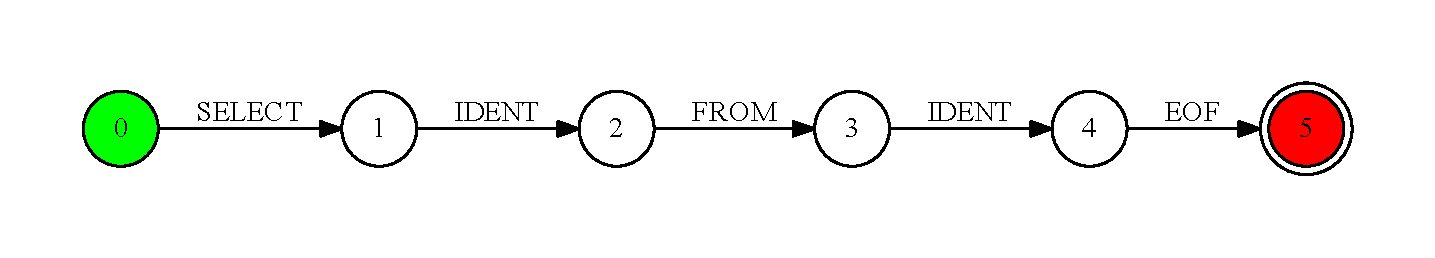
\includegraphics[width=1.0\linewidth]{TokenEx}
\end{center}

\item Конечный автомат первого токена \verb|IDENT|:
\begin{center}
   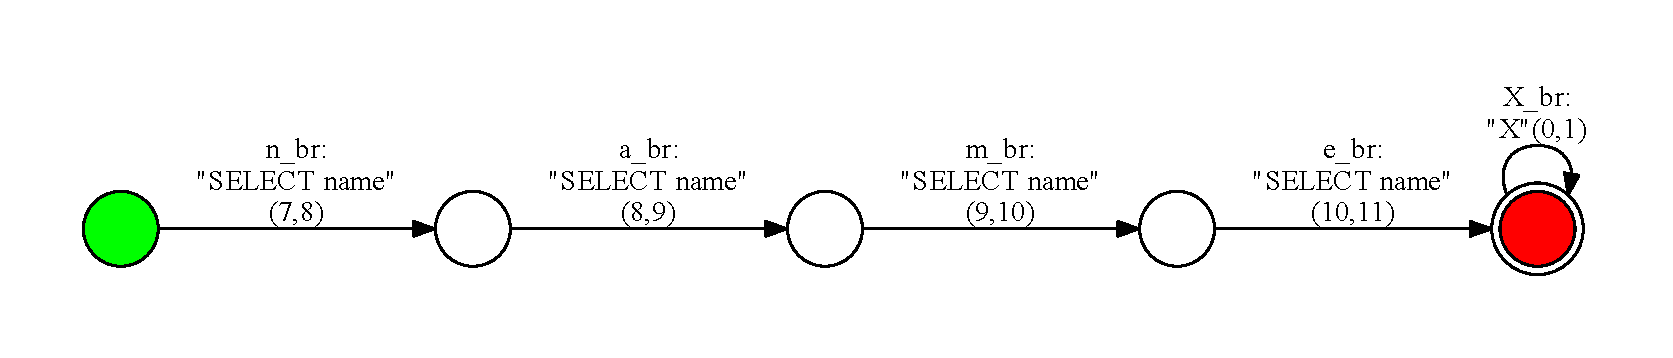
\includegraphics[width=1.0\linewidth]{token}
\end{center}
\end{itemize}
\end{frame}


\begin{frame}[fragile]
\transwipe[direction=90]
\frametitle{Результаты}
В рамках данной работы были получены следующие результаты:
\begin{itemize}
\item Разработан алгоритм лексического анализа выражений, формируемых с помощью строковых операций и циклов
\item Реализован генератор лексических анализаторов на основе предложенного алгоритма
\end{itemize}
\end{frame}


\begin{frame}
\transwipe[direction=90]
\frametitle{Область применения}
\begin{itemize}
\item Реинжиниринг программного обеспечения
	\begin{itemize}
	\item Анализ и трансформация систем, использующие строковые выражения
	\end{itemize}
\item Поддержка строковых выражений в IDE
	\begin{itemize}
    \item Статический поиск ошибок
	\item Подсветка синтаксиса
	\item Рефакторинг
	\end{itemize}
\end{itemize}
\end{frame}

\begin{frame}
\transwipe[direction=90]
\frametitle{Контактная информация}
\begin{itemize}
\item Полубелова Марина: polubelovam@gmail.com
\item Григорьев Семён: Semen.Grigorev@jetbrains.com
\item Исходный код YaccConstructor:
\href{https://github.com/YaccConstructor}{https://github.com/YaccConstructor}
\end{itemize}
\end{frame}

\end{document}
